\section{Related Work}
\label{sec:related_work}

In this chapter, we have chosen two papers to relate theories from to our business idea and the Watchr media platform. The papers in question are: "\textit{The Early Stage Software Startup Development Model: A Framework for Operationalizing Lean Principles in Software Startups.}" (Bosch, Bjork and Ljungblad) and "\textit{The Nature of the Entrepreneurial Process: Causation, Effectuation, and Pragmatism.}"(Kraaijenbrink). 

\subsection{The ESSSDM}

Contrary to popular believe, many software start-ups fail in their inception and there are only a very few that manage to become very successful (Facebook, Twitter, Instagram to name a few). In order to identify what factors contribute to the success of a software start-up, we first have to understand what constitutes one. According to Ries \todo{(ref here)}, a "\textit{startup is a human institution designed to deliver a new product or service under conditions of extreme uncertainty}". Additionally, many start-ups usually have limited resources in terms of people and funding at their disposal which strengthens the importance of minimizing the development time and effort while maximizing the value. Lean principles emphasize on continuous learning through customer validation and short feedback cycles to identify which efforts or activities generate customer value.


In order to address that, we would make use of the Early Stage Software Startup Development Model (ESSSDM) and elaborate on each of its comprising parts. This model allows the exploration of multiple ideas in parallel and evaluating the ones worth scaling through short iterative cycles (using the Build-Measure-Learn loop). It consists of three parts: 
  
\begin{figure}[h]
\begin{center}
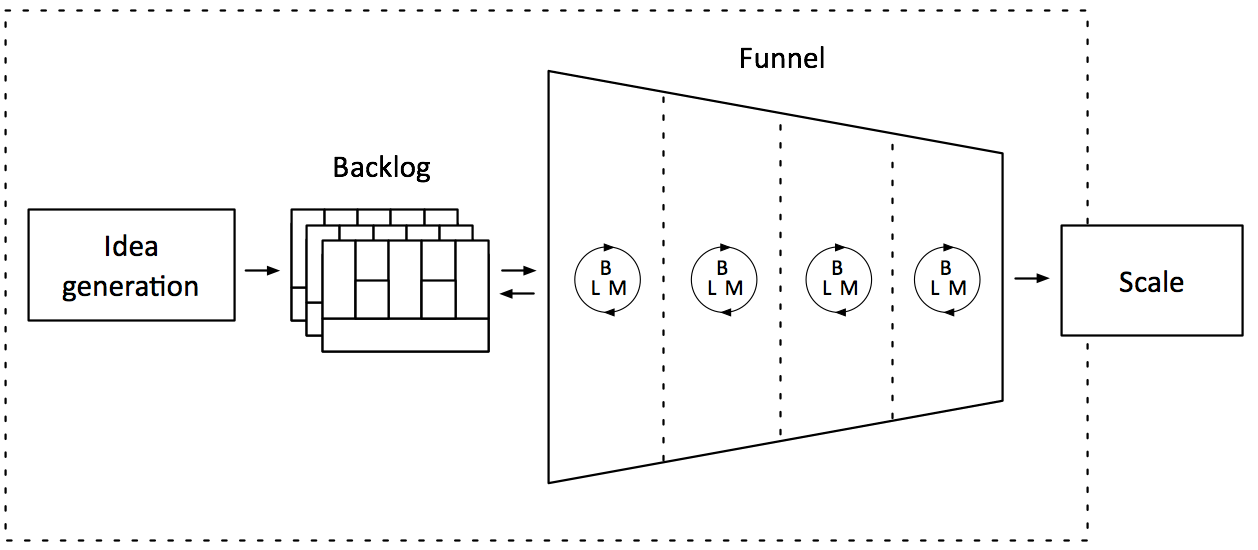
\includegraphics[scale=0.55]{./pics/ESSSDM}
\caption{Early Stage Software Startup Development Model}
\label{fig:esssdm}
\end{center}
\end{figure}
\begin{enumerate}

\item Idea generation

This stage is considered a part of the startup process and happens prior to incorporation. In our case, we started by brainstorming several possible avenues we can pursue before eventually settling on building a online media streaming platform which would incorporate some elements from already existing such platforms (content filtering by different criteria, recommended,popular and favourite lists,rating system etc.). 
\item Ideas backlog

Here is where all the ideas generated are put into a prioritized backlog. It is really important that they are written in comparable format otherwise the prioritization  becomes extremely complex. Some other product ideas we have included: a so-called "Omni compiler" which would conceptually translate legacy COBOL code, heavily used in the financial sector and with a high demand, into a modern language with higher maintainability and lower operation costs and potentially a mobile game with a competitive nature given the current high market demand.
\item The Funnel

The last stage of the ESSSDM entails how multiple ideas are fed into a "funnel" where they undergo a validation systematically by the use of the Build-Measure-Learn (BML) loop. Multiple ideas can be in the funnel while being validated in parallel. This is worthwhile since it is really important to stay objective in the early stages of a startup. This gives an open mind and willingness to change instead of sticking and growing attached to one single idea which might be damaging that early on. This stage consists of four sub-stages: (1) Validate problem, (2) Validate solution, (3) Validate Minimum Viable Product (MVP) small-scale, and (4) Validate Minimum Viable Product (MVP) large-scale but we have only discussed hypothetically how we are going to address these stages since coming up with a solution, its validation and a minimum viable product is beyond the scope of this project.
 \end{enumerate}
 
